\documentclass[handout]{beamer}
\usepackage[orientation=portrait,size=A4]{beamerposter} 

\usepackage[utf8]{inputenc}
\usepackage[T1]{fontenc}
\usepackage{fontspec}
\usepackage[french]{babel}
\usepackage{graphicx}
\usepackage{array}
\usepackage{pifont}
\usepackage{amsmath, amssymb}

\newcommand{\tick}{\ding{52}}

\graphicspath{ {./images/} }


\newcommand{\ensemble}[1]{\left\lbrace{} #1 \right\rbrace{}}

%\usetheme{Boadilla}

\title{Optimisation de circuits logiques}

\author{Alexandre JANNIAUX}

\begin{document}

\begin{frame}
  \maketitle
  \tableofcontents
\end{frame}

\section{Circuits logiques et fonctions combinatoires}
\begin{frame}
  \frametitle{Circuits logiques et fonctions combinatoires}
  \begin{figure}[p]
    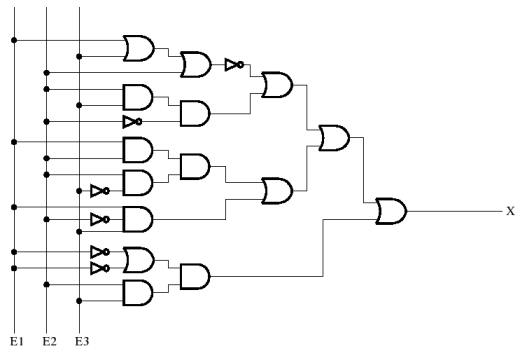
\includegraphics[width=8cm]{circuit_logique.png}
    \caption{Exemple de circuit logique}
    \label{fig:circ1}
  \end{figure}
  
  \[ \begin{aligned}
    f: \ensemble{0,1}^3 &\longrightarrow & \ensemble{0,1} \\
    (e_1,e_2,e_3) & \longmapsto & f(e_1,e_2,e_3) 
  \end{aligned}
  \]
  
  \begin{figure}[p]
%    \input{'graph_rec.tex'}
  \end{figure}
  

  
\end{frame}

\section{M\'ethode de Quine-McCluskey}
\begin{frame}
  \frametitle{M\'ethode de Quine-McCluskey}

  \[ \mathcal{F} = f^{-1}({1}) \]
  
  \begin{figure}[p]
    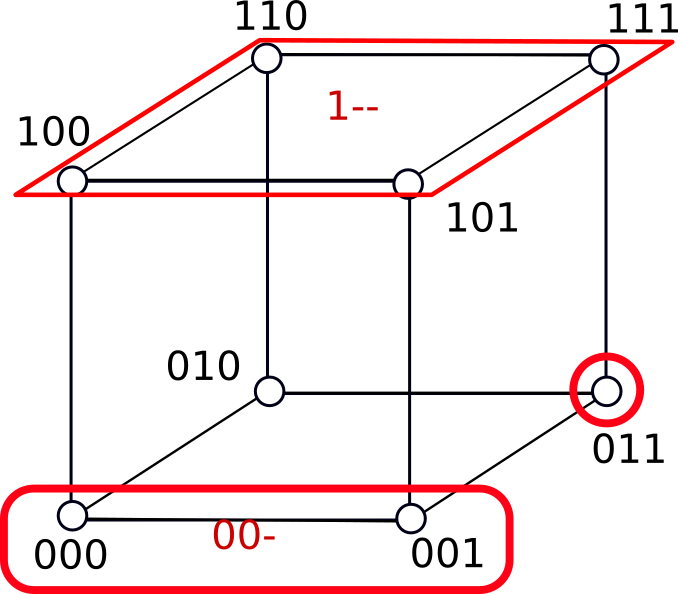
\includegraphics[width=8cm]{cube_qm.png}
    \caption{Repr\'esentation graphique de minterme}
    \label{fig:cube1}
  \end{figure}
  
  \large{\textbf{Exemple :}} \[ f(x_1,\cdots,x_6) = \sum m(36, 44, 51, 60) \]
  
  %\begin{minipage}
    \begin{tabular}{rl}
      36: & 100100  \tick \\ \hline 
      44: & 101100  \tick \\ 
      51: & 110011   \\ \hline
      60: & 111100 \tick
    \end{tabular}
  %\end{minipage}

  %\begin{minipage}
    \begin{tabular}{rl}
      36,44: & 10\_100  \\ \hline 
      44,60: & 1\_1100    
    \end{tabular}
  %\end{minipage}
  
  %\large{\textbf{Idée :}} Une fonction combinatoire est définie par le langage accepté (couverture).
  
  %=> On utilise l'algèbre de Boole pour simplifier les expressions
  
  %\large{\textbf{Algorithme :}}
  %\begin{enumerate}
  %   \item 
  %\end{enumerate}
\end{frame}

\section{M\'ethode de Petrick}
\begin{frame}
  \frametitle{M\'ethode de Petrick}
 
  Couverture d'ensemble minimale.

  \begin{tabular}{|l|c|c|c|c|}
    \hline %
    Implicants & 36 & 44 & 51 & 60  \\ \hline
    51 &  &  & X &  \\ \hline
    36,44 & X & X &  &    \\ \hline
    44,60 &  & X &  & X \\ \hline
  \end{tabular}
  
  \begin{itemize}
  \item Redondance
  \end{itemize}
\end{frame}

\section{Fonctions multivaluées}
\begin{frame}
  \frametitle{Fonctions multivaluées}

  \textbf{Définition :}
  \[ f: \mathcal{P}_1 \times \cdots \times \mathcal{P}_n \longrightarrow \mathbb{B}^m \]

  \textbf{Littéraux :} 

  \[X_i^{S_i} = %
  \begin{cases}
    1 \text{ si } X_i \in S_i$ \\
    0 \text{ sinon}
  \end{cases}
  \quad \text{où } X_i \in \mathcal{P}_i \text{ et } \mathcal{S}_i \subset \mathcal{P}_i \]

  \textbf{Décomposition de Shannon :}

  \[ \bigcup_{i=1}^n c_i = 1 \implies f \equiv \bigcup_{i=1}^{n} f\,|_{C_i} \cap c_i \]

\end{frame}

\begin{frame}
  \frametitle{Espresso}

  \textbf{Initialisation :}
  
  \begin{itemize}
  \item Expension
  \item Élimination des redondances
  \item Recherche des impliquants essentiels
  \end{itemize}

  \textbf{Algorithme :}
  % Tant qu'on peut le faire : 
  \begin{itemize}
  \item Réduction
  \item Expension
  \item Élimination des redondances
  \end{itemize}
  
\end{frame}

\end{document}
